Using feedback from the force-torque sensors the Hubo-Ach controller adds compliance to the legs via active damping.
Fig.~\ref{fig:activedamping} shows as the user pushes down on the robot the force is detected by the force-torque (FT) sensors.
This then modifies the joint commands such that the center of mass (CoM) acts like there is an over-damped spring-damper system between it and mechanical ground.

\footnotesize
\noindent \textbf{Python Source Code for Active Damping using force-torque sensors}
\vspace{-6mm}
\begin{code}

#!/usr/bin/env python
# /* -*-  indent-tabs-mode:t; tab-width: 8; c-basic-offset: 8  -*- */
import hubo_ach as ha
import ach
import sys
import time
from ctypes import *

# Open Hubo-Ach feed-forward and feed-back (reference and state) channels
s = ach.Channel(ha.HUBO_CHAN_STATE_NAME)
r = ach.Channel(ha.HUBO_CHAN_REF_NAME)
s.flush()
r.flush()

# feed-forward will now be refered to as "state"
state = ha.HUBO_STATE()

# feed-back will now be refered to as "ref"
ref = ha.HUBO_REF()

g = 0.4
kz = 0.28

imax = 10
delta = g/imax
for i in range(1, imax):
  ref.ref[ha.RAP] = -delta*i
  ref.ref[ha.LAP] = ref.ref[ha.RAP]
  ref.ref[ha.RKN] = 2*delta*i
  ref.ref[ha.LKN] = ref.ref[ha.RKN]
  ref.ref[ha.RHP] = -delta*i
  ref.ref[ha.LHP] = ref.ref[ha.RHP]

  r.put(ref)
  time.sleep(0.1)

d = 0.0
L = 5.0
while True:
  # Get the current feed-forward (state) 
  [statuss, framesizes] = s.get(state, wait=False, last=False)
  ft = (state.ft[ha.HUBO_FT_R_FOOT].f_z + state.ft[ha.HUBO_FT_L_FOOT].f_z)/2.0/200.0
  dt = kz*ft
  d = (d*(L-1.0)+dt)/L

  if d > 0.4: 
    d = 0.4
  if d < -0.4:
    d = -0.4

  ref.ref[ha.RAP] = -(g+d)
  ref.ref[ha.LAP] = ref.ref[ha.RAP]
  ref.ref[ha.RKN] = 2*(g+d)
  ref.ref[ha.LKN] = ref.ref[ha.RKN]
  ref.ref[ha.RHP] = ref.ref[ha.RAP]
  ref.ref[ha.LHP] = ref.ref[ha.RHP]

#  ref.ref[ha.REB] = g + ky*state.ft[ha.HUBO_FT_R_HAND].m_y
  print 'New Ref: ', ref.ref[ha.RKN], ' d = ', d, ' dt = ', dt

  # Write to the feed-forward channel
  r.put(ref)

  time.sleep(0.05)  

# Close the connection to the channels
r.close()
s.close()
\end{code}
\normalsize

\begin{figure}[thpb]
  \centering
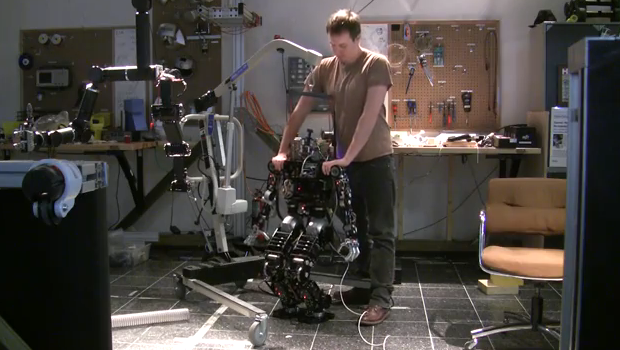
\includegraphics[width=0.6\columnwidth]{./pix/activedamping.png}

\includegraphics[width=0.3\columnwidth]{./qrcode/qrcode-activedamping.png}\\
     http://danlofaro.com/phd/activedamping/
  \caption{Using feedback from the force-torque sensors the Hubo-Ach controller adds compliance to the legs via active damping. }
  \label{fig:activedamping}
\end{figure}
